% !TeX root = ../../main.tex
\resizebox{\textwidth}{\textwidth}{
    \tikzsetnextfilename{reconstruct_point1}
    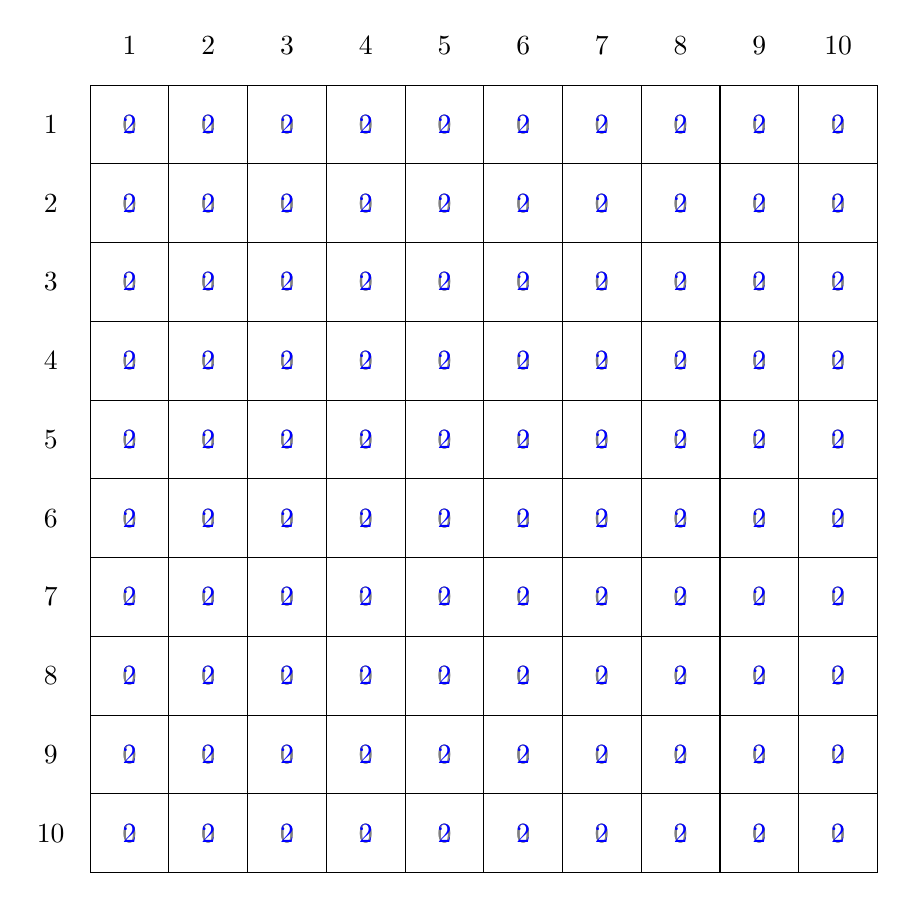
\begin{tikzpicture}
    \foreach \x in {1,...,10} {
        \draw (\x + 0.5, 11.5) node {\x};
    }
    \foreach \y in {10,...,1} {
        \draw (0.5, 11.5 - \y) node {\y};
    }
    \foreach \x in {1,...,10} {
        \foreach \y in {1,...,10} {
            \draw (\x, \y) rectangle (\x +1, \y +1);
            \ifnumcomp{\x}{<}{3}{
                \draw[color=gray] (\x +0.5, \y +0.5) node {0};
            }{
                \ifnumcomp{\y}{>}{7}{
                    \draw[color=gray] (\x +0.5, \y +0.5) node {0};
                }{
                    \draw[color=blue] (\x +0.5, \y +0.5) node {2};
                }
            }
        }
    }
    \end{tikzpicture}
}